\section{Korrelationsmatrizen sortiert nach dem Gemeindeschlüssel}
\subsection{Korrelationsmatrizen mit den nach Gemeindeschlüsseln sortierten Landkreisen}
In \autoref{fig:matrizes_north_to_south_counties} befinden sich die sechs Matrizen mit den Werten für die Korrelationen zwischen den Landkreisen.
Die Zeilen und Spalten sind lexikographisch nach den Gemeindeschlüsseln der Landkreise sortiert und diesen zugeordnet. In \autoref{tab:counties_by_admunitid} befindet sich die komplette sortierte Liste der Landkreise.
\begin{figure}[H]
    \centering
    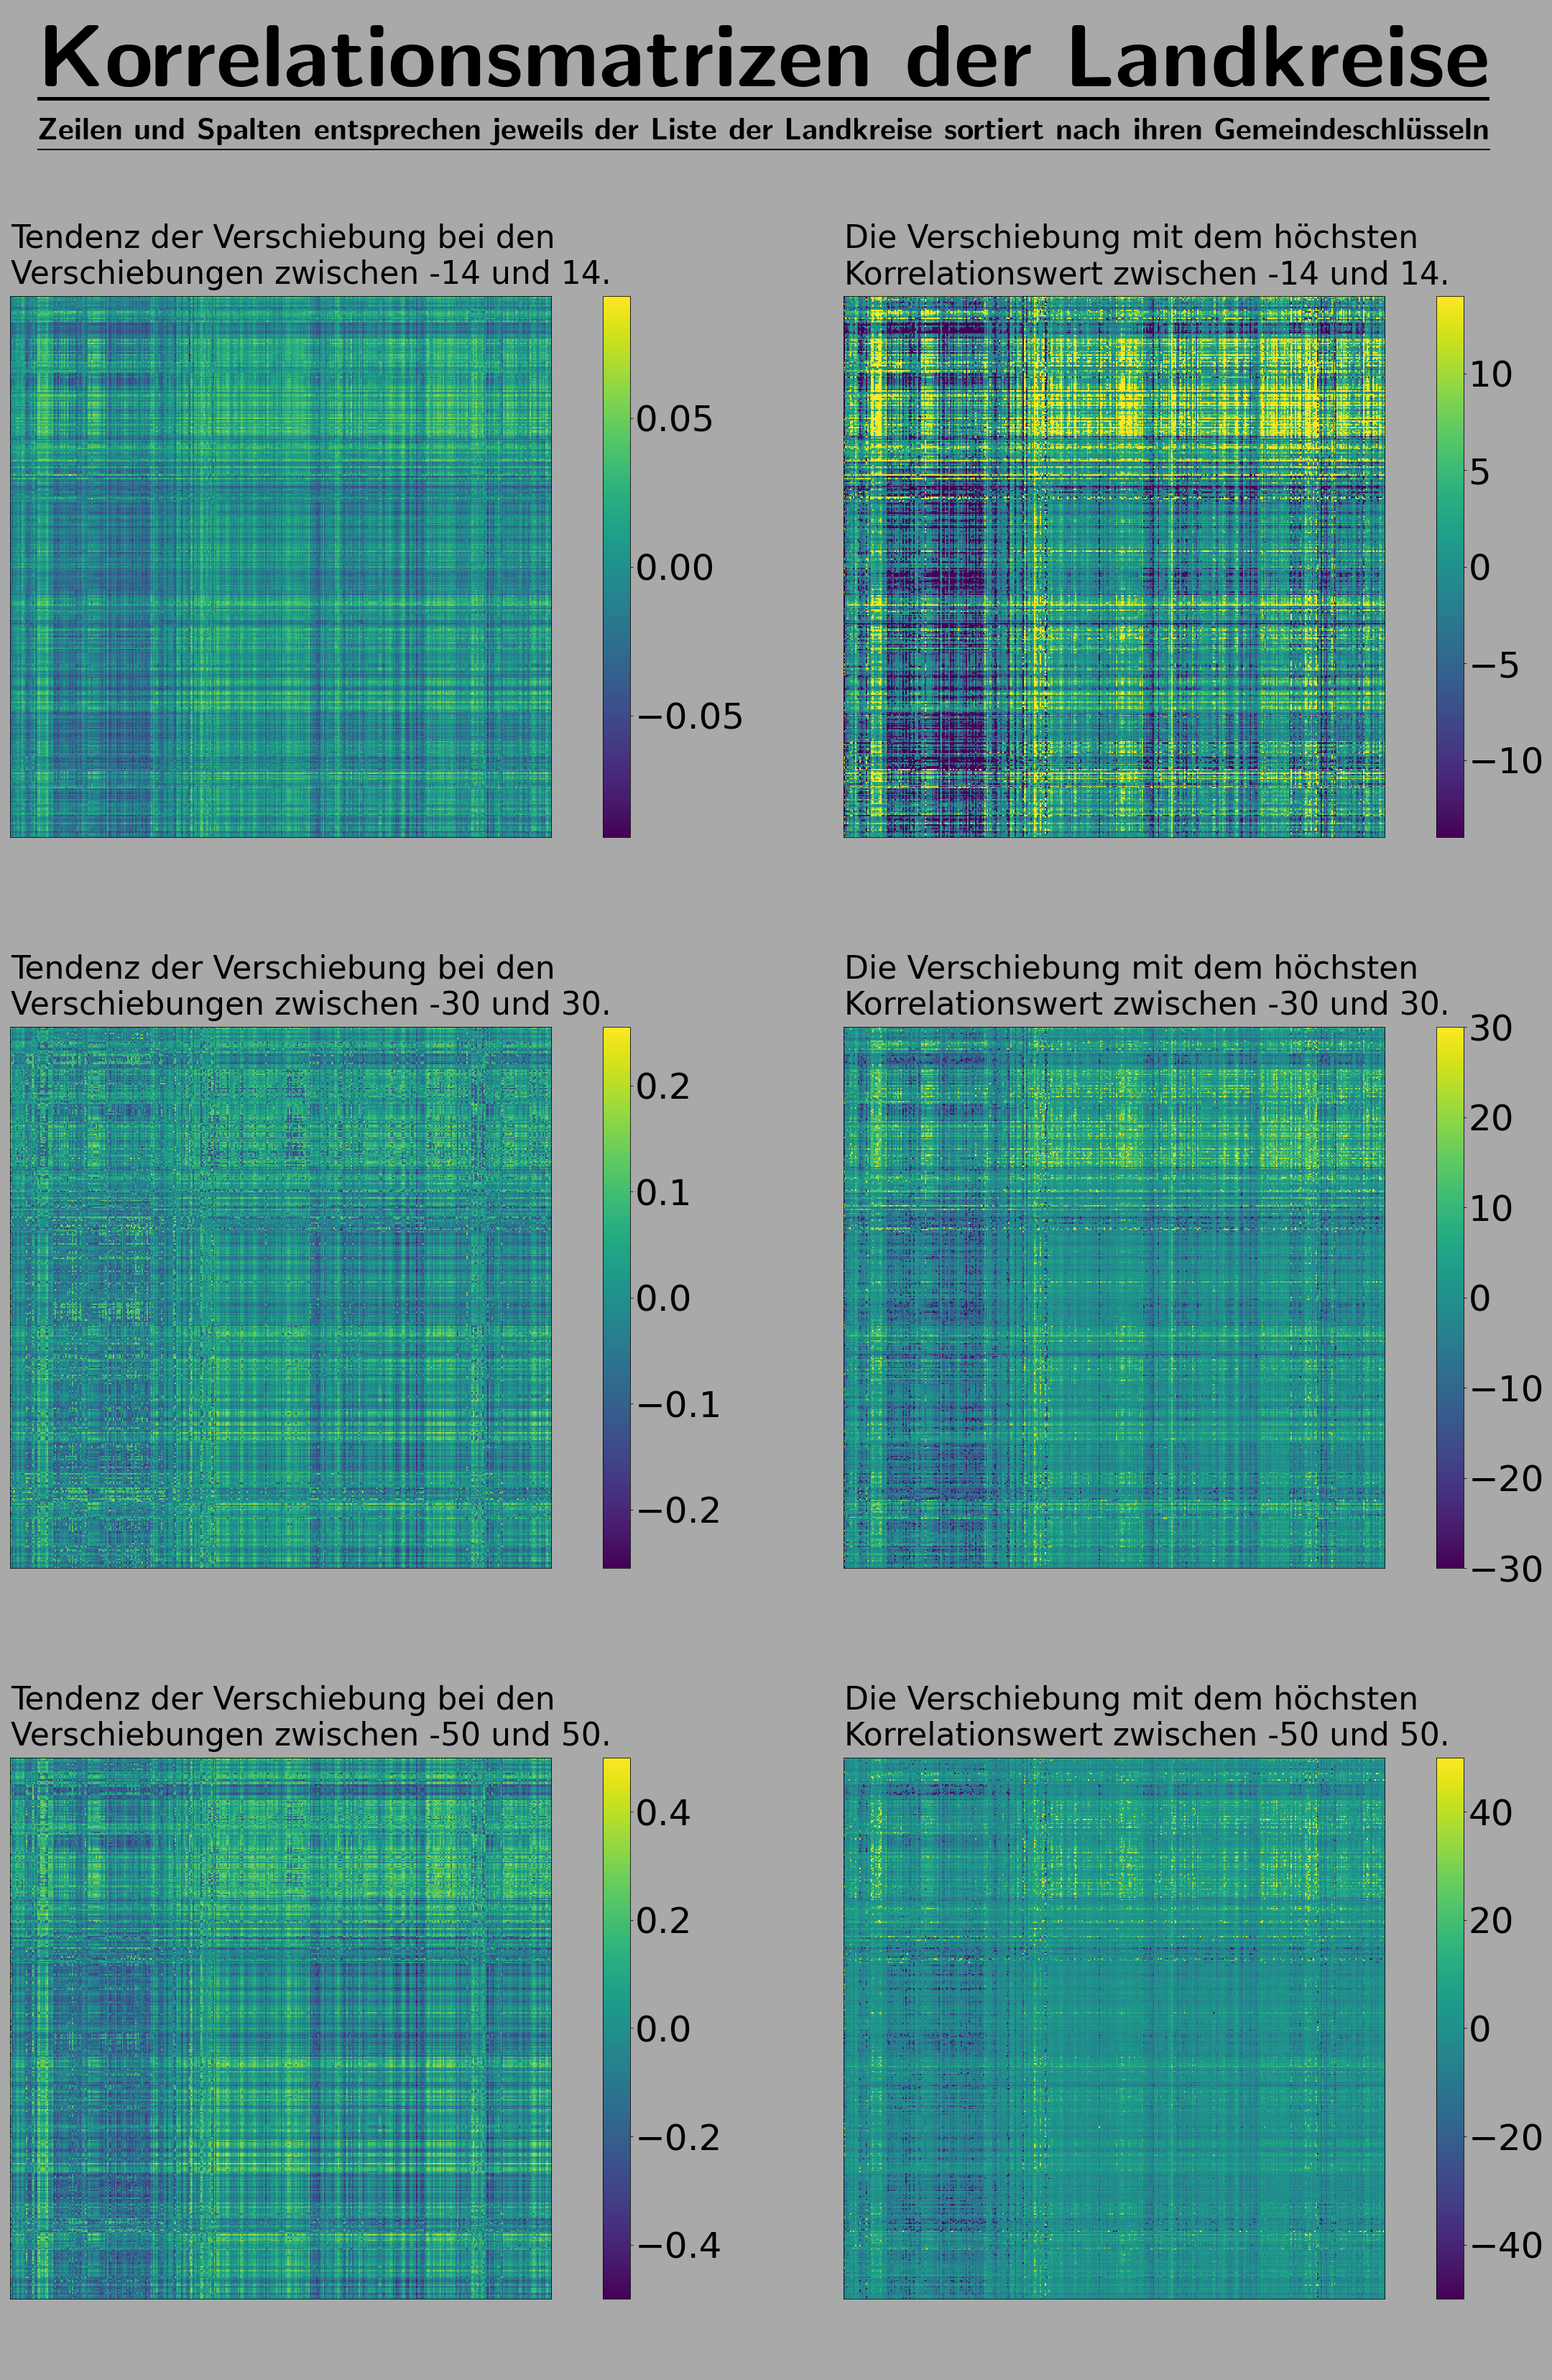
\includegraphics[width = \textwidth]{figures/Ergebnisse/matrizes_north_to_south_counties.png}
    \caption{Korrelationsmatrizen der Korrelationen aller Landkreise zeilen- und spaltenweise nach dem Gemeindeschlüssel sortiert (siehe \autoref{tab:counties_by_admunitid}). Die Farben der Zellen der linken Matrizen entsprechen den Tendenzen der Verschiebung des Landkreises der Spalte in Relation zum Landkreis der Zeile.
    Auf der rechten Seite wir die Zelle entsprechend der Verschiebung der Zeitreihe des Landkreises der Spalte entgegen der Zeitreihe der Zeile mit dem höchsten Korrelationswert eingefärbt. Beide Vorgehensweise werden für alle Verschiebungen $\tau\in[-14,14]$,  $\tau\in[-30,30]$ und  $\tau\in[-50,50]$ durchgeführt und in dieser Reihenfolge von oben nach unten dargestellt.}
    %\label{fig:matrizes_north_to_south_counties}
\end{figure}

\begin{figure}[H]
    \centering
    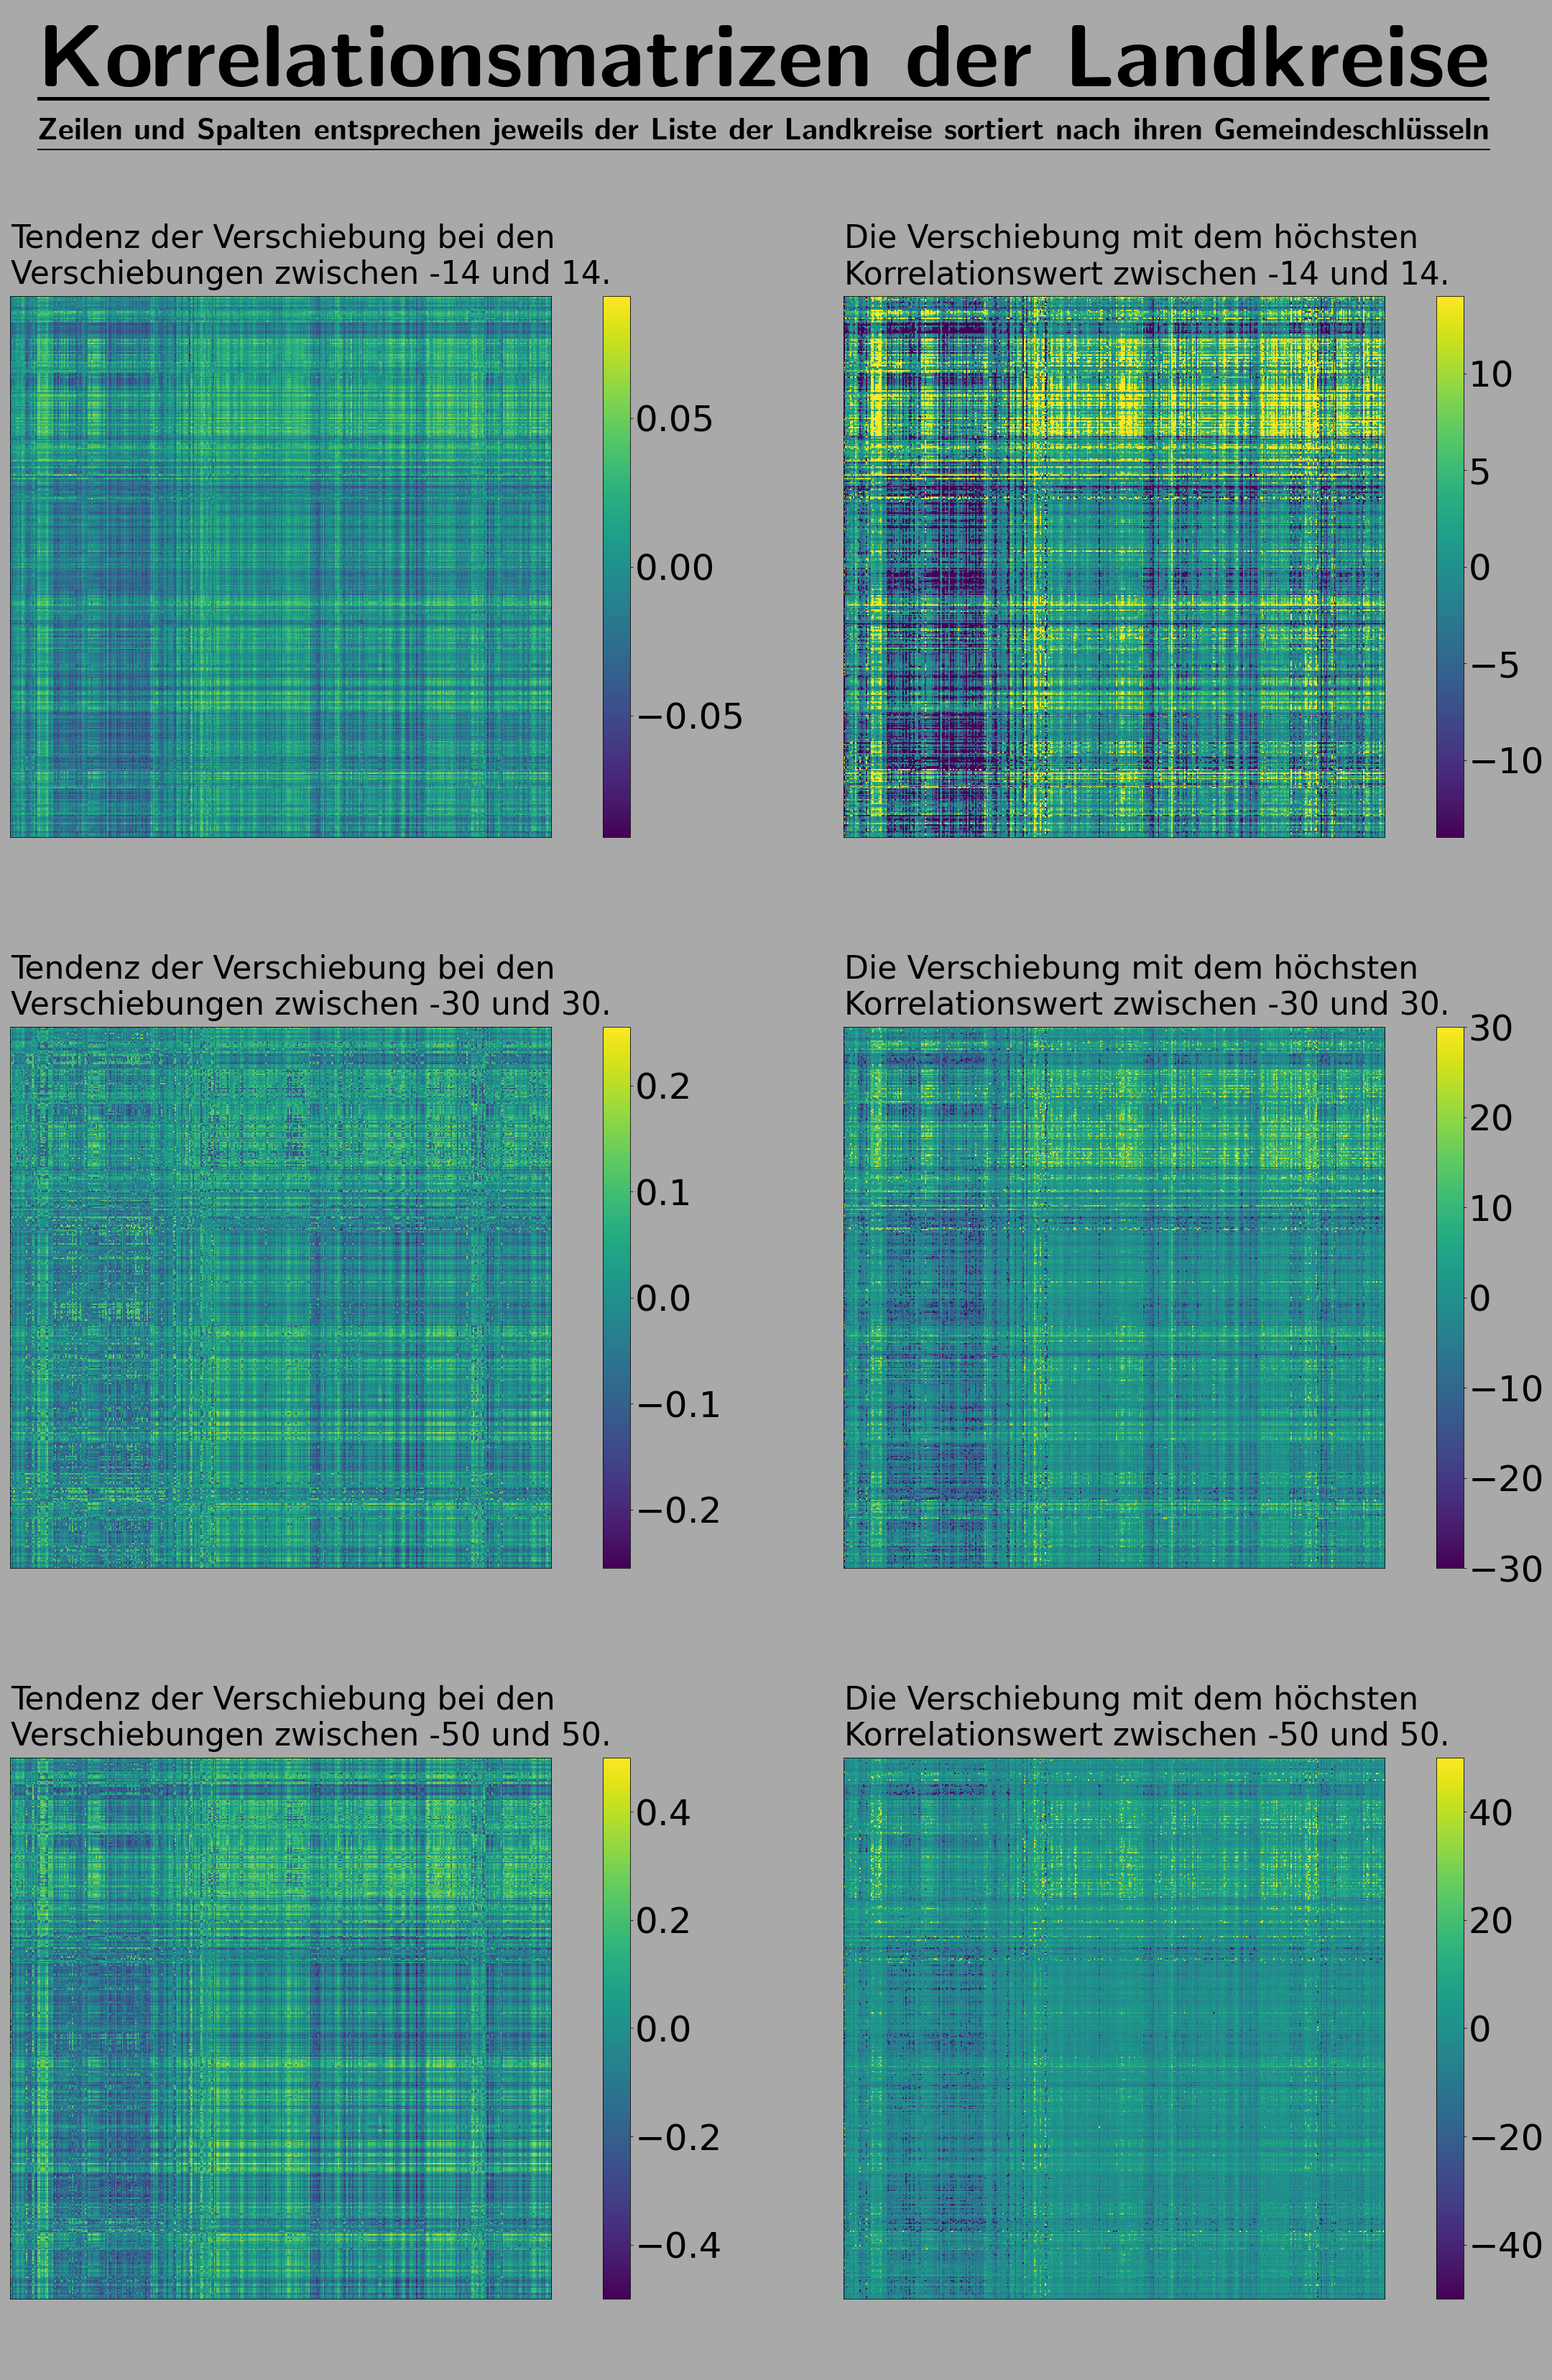
\includegraphics[width = 0.75\textwidth]{figures/Ergebnisse/matrizes_north_to_south_counties.png}
    \caption{Korrelationsmatrizen der Korrelationen aller Landkreise zeilen- und spaltenweise nach dem Gemeindeschlüssel sortiert (siehe \autoref{tab:counties_by_admunitid}). Die Farben der Zellen der linken Matrizen entsprechen den Tendenzen der Verschiebung des Landkreises der Spalte in Relation zum Landkreis der Zeile.
    Auf der rechten Seite wir die Zelle entsprechend der Verschiebung der Zeitreihe des Landkreises der Spalte entgegen der Zeitreihe der Zeile mit dem höchsten Korrelationswert eingefärbt. Beide Vorgehensweise werden für alle ganzzahligen Verschiebungen $\tau\in[-14,14]$,  $\tau\in[-30,30]$ und  $\tau\in[-50,50]$ durchgeführt und in dieser Reihenfolge von oben nach unten dargestellt.}
    \label{fig:matrizes_north_to_south_counties}
\end{figure}
\subsection{Korrelationsmatrizen mit den nach Gemeindeschlüsseln sortierten Regierungsbezirken}

\begin{figure}[H]
    \centering
    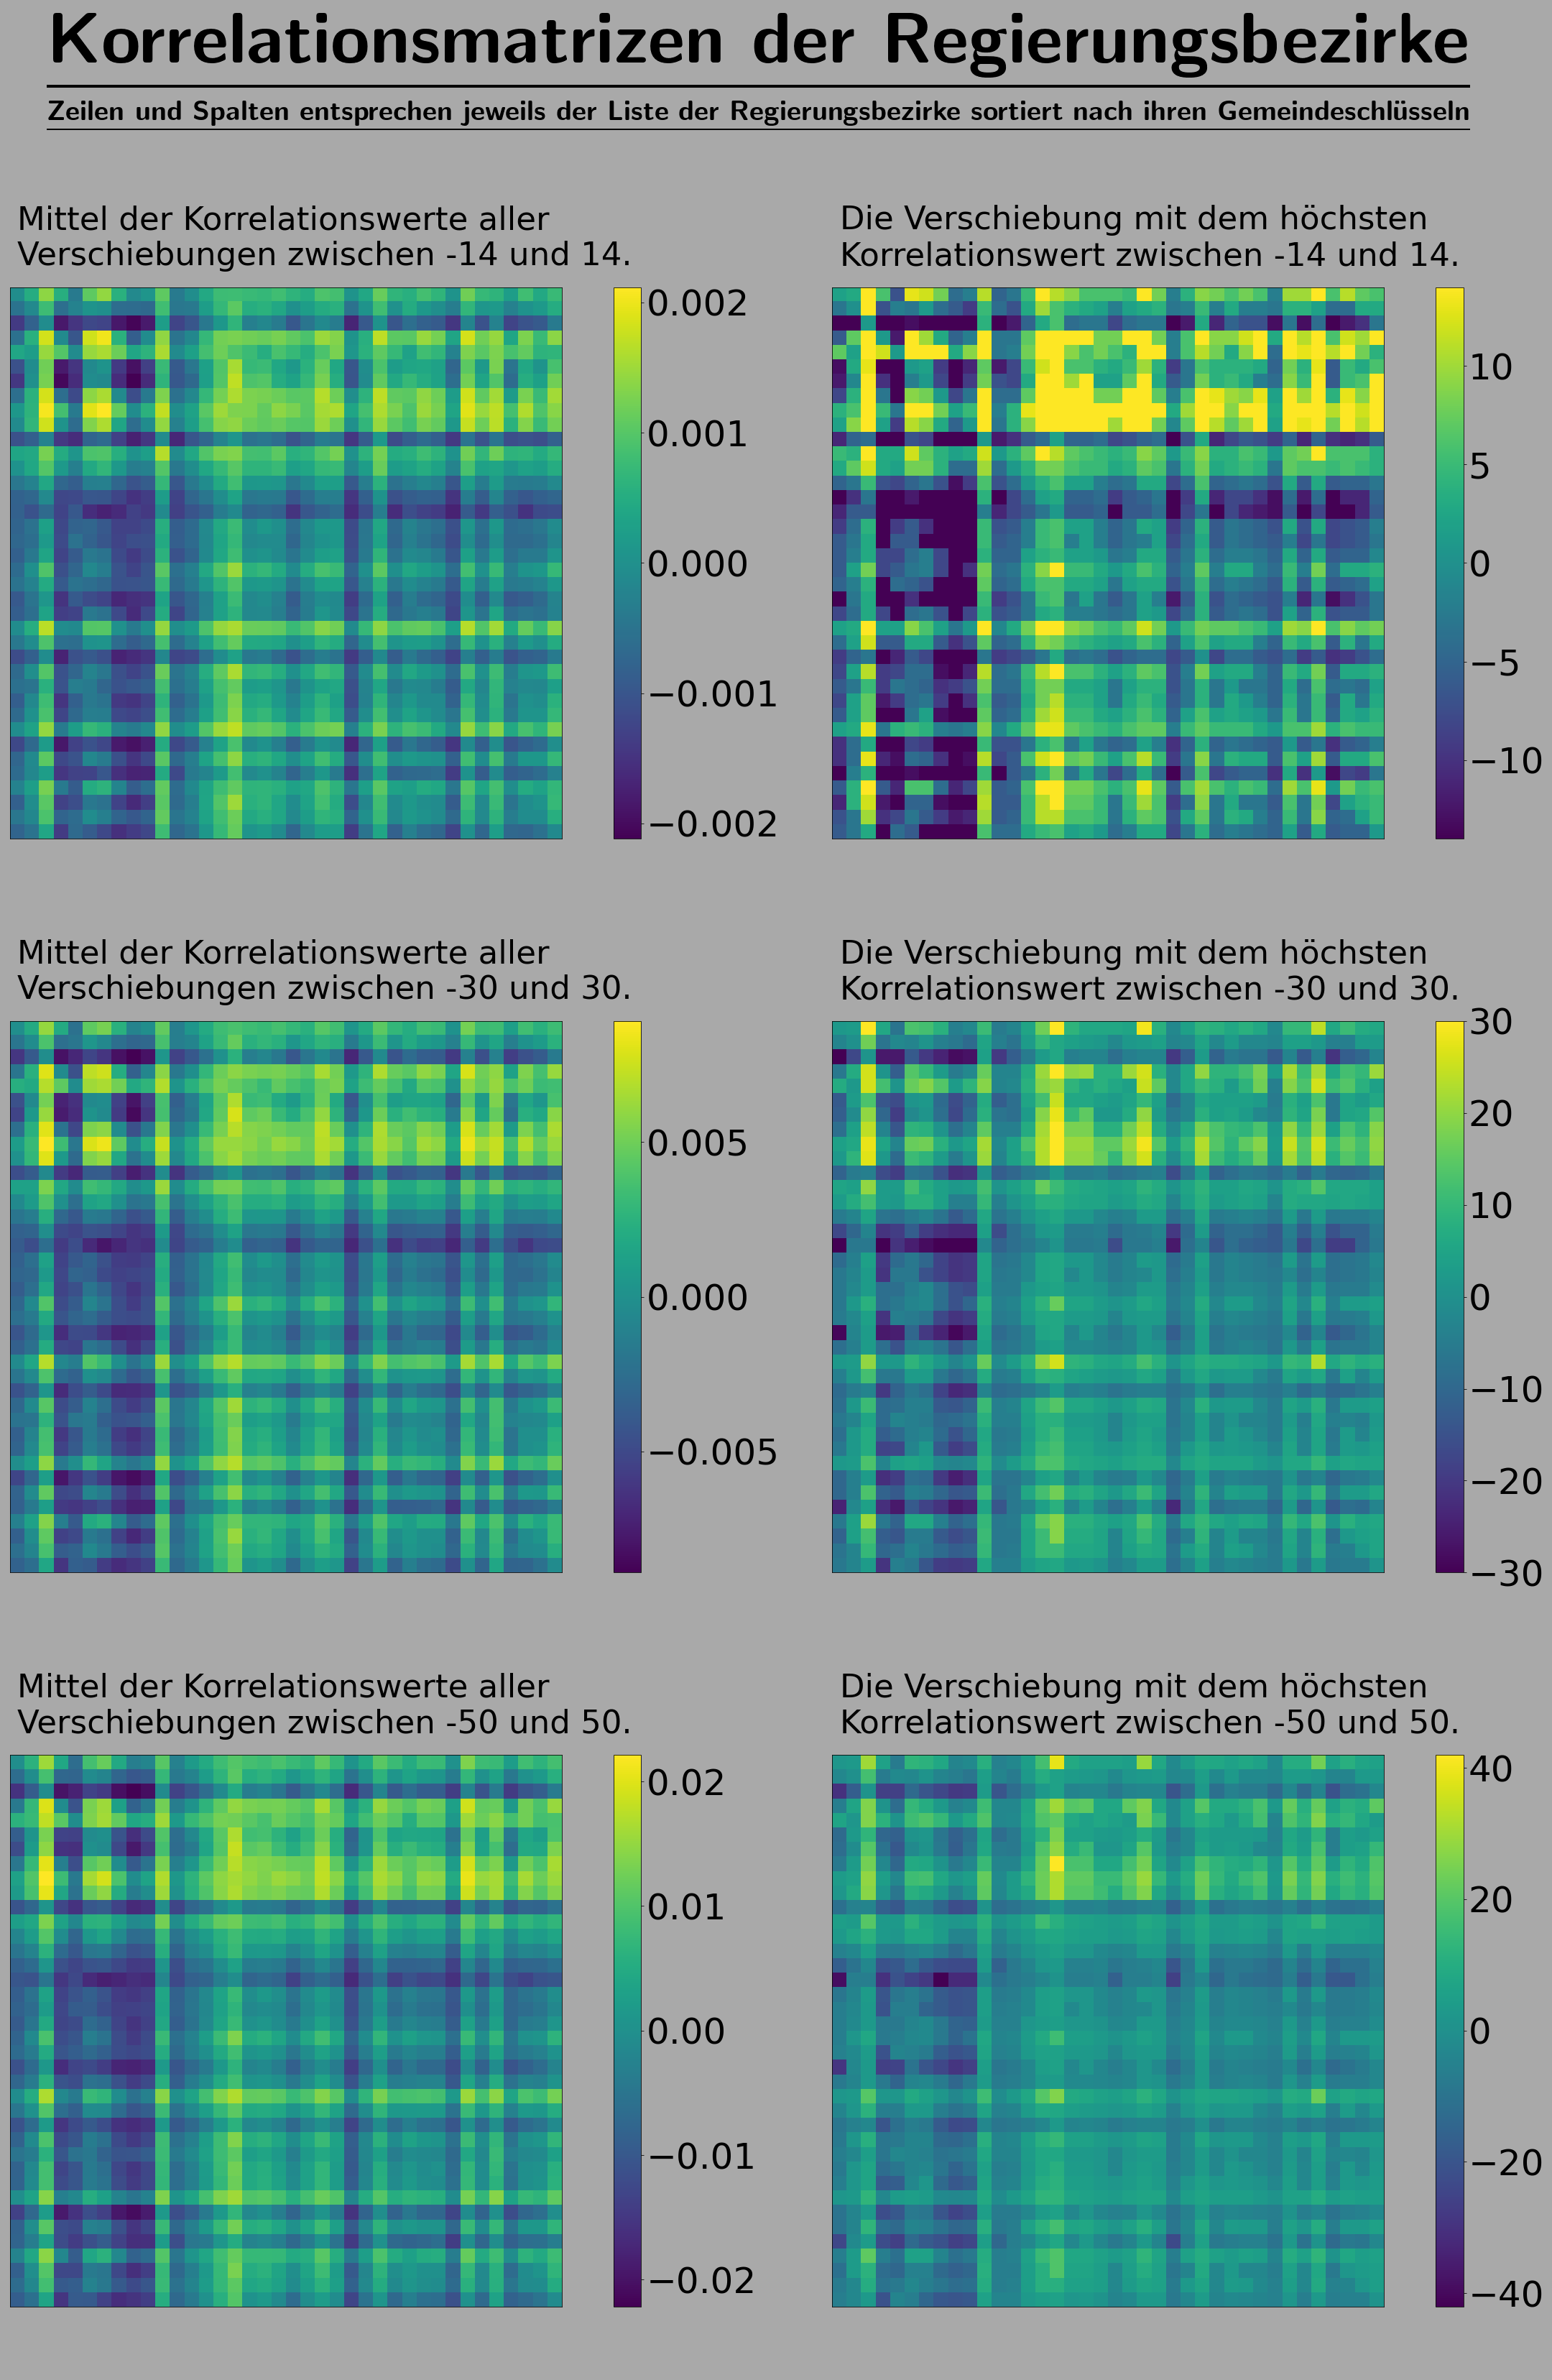
\includegraphics[width = \textwidth]{figures/Ergebnisse/matrizes_north_to_south_districts.png}
    \caption{Korrelationsmatrizen mit den nach Gemeindeschlüsseln sortierten Regierungsbezirken, wie in \autoref{sec:Vorgehensweise:Korrelationsanalysen aller Landkreise und Regierungsbezirke} beschrieben. Die Regierungsbezirke sind den Zeilen und Spalten in lexikographischer Ordnung ihrer Gemeindeschlüssel-Präfixe zugeordnet, siehe \autoref{tab:districts_by_admunitid}.\\
    Die Zellen sind gemäß der Verschiebung $\tau_0$ in Tagen mit dem maximalen Wert $c(\tau_0)$ (\autoref{sec:Grundlagen:Korrelation:Komprimierung}) oder der Tendenz der Verschiebung $\hat{\tau}$ (\autoref{eq:Tendenz der Verschiebung}) eingefärbt. Die beiden Kennzahlen werden für die Verschiebungen $\tau$ in den Intervallen $[-14, 14]$, $[-30, 30]$ und $[-50,50]$ ermittelt und beziehen sich auf die Verschiebung des Regierungsbezirks der Spalte in Relation zu dem der Zeile.
    }
    \label{fig:matrizes_north_to_south_districts}
\end{figure}

Die sechs Matrizen mit den Werten für die Korrelationen zwischen den Regierungsbezirken befinden sich in \autoref{fig:matrizes_north_to_south_districts} . Auch hier sind die Zeilen und Spalten lexikographisch nach den Gemeindeschlüsseln der Landkreise in den Regierungsbezirken sortiert. Die vollständige Auflistung von diesen befindet sich im Anhang in \autoref{tab:districts_by_admunitid}.